%!TEX root = ../username.tex
\chapter{Realtime Audio Programming}
\hspace*{-0.155cm}This chapter will consider the theory behind audio programming and the different principles that are followed to create a functional program.
\section{Sound As A Discrete Signal}
Sound is a physical phenomenon. Differences in air pressure are picked up by tiny hairs inside ears, which is converted to []. Naturally, representing this in a digital setting involves .

\begin{figure}[h] % [h] used to prevent {figure} from doing weird positioning
\begin{center}
	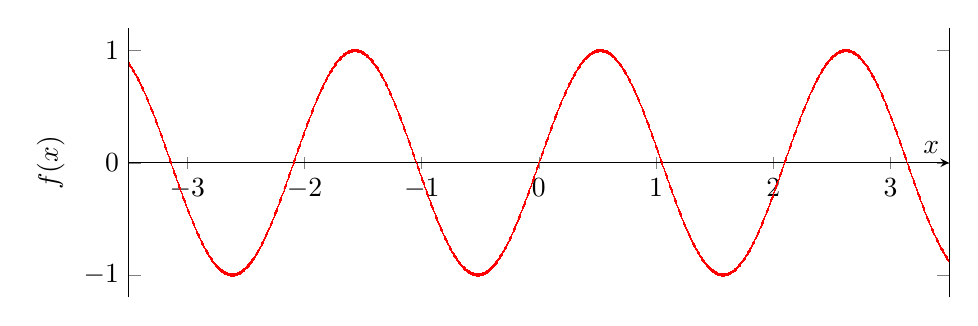
\begin{tikzpicture}
		\begin{axis} [
			axis x line = middle, % The x axis should go through the origin
			xlabel = \(x\),
			ylabel = {\(f(x)\)},
			height = 5cm,
			width = 12cm
			]

			\addplot [
			jump mark mid,
			domain = -3.5:3.5,
			samples = 1000,
			very thick, red
			] {(sin(deg(3 * x)))};

		\end{axis}
	\end{tikzpicture}
	\caption{A graph of the sine wave \(f(x) = sin(3x)\).}
\end{center}
\end{figure}

\section{The Realtime Programming Bus Schedule}
[] Unlike a music player, our program has to follow the set schedule requested by the audio driver of a device [].
\section{Technical Details}
\section{Obstacles to Overcome}
\section{The VST Software Development Kit}
